\begin{figure}[htbp]
    \centering
    \resizebox{0.92\textwidth}{!}{%
    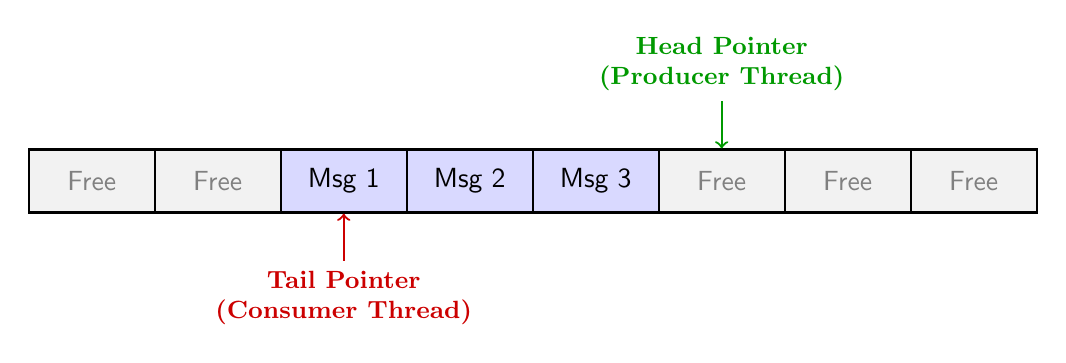
\begin{tikzpicture}[
        font=\sffamily,
        cell/.style={rectangle, draw=black, thick, minimum width=1.6cm, minimum height=0.8cm, align=center},
        used/.style={cell, fill=blue!15},
        free/.style={cell, fill=gray!10, text=gray},
        arrow/.style={->, thick, >=stealth}
    ]

    % Array cells
    \node[free] (c0) at (0, 0) {Free};
    \node[free] (c1) at (1.6, 0) {Free};
    \node[used] (c2) at (3.2, 0) {Msg 1};
    \node[used] (c3) at (4.8, 0) {Msg 2};
    \node[used] (c4) at (6.4, 0) {Msg 3};
    \node[free] (c5) at (8.0, 0) {Free};
    \node[free] (c6) at (9.6, 0) {Free};
    \node[free] (c7) at (11.2, 0) {Free};

    % Pointers
    \draw[<-, thick, color=red!80!black] (c2.south) -- +(0, -0.6) node[below, align=center, font=\bfseries\small] {Tail Pointer\\(Consumer Thread)};
    \draw[<-, thick, color=green!60!black] (c5.north) -- +(0, 0.6) node[above, align=center, font=\bfseries\small] {Head Pointer\\(Producer Thread)};

    \end{tikzpicture}%
    }
    \caption{A lock-free Single-Producer Single-Consumer (SPSC) ring buffer. The producer actively writes to the Head pointer while the consumer asynchronously trails behind reading from the Tail pointer. Because the two threads concurrently modify distinct atomic variables, they operate entirely lock-free. So long as the underlying logic uses safe modulo arithmetic to wrap edges, the system remains infinitely scalable for isolated threads.}
    \label{fig:spsc_queue}
    \vspace{1em}
\end{figure}
